\chapter{Methods and Resources}
\label{chap:methods}

%\section{Overview/meta-text}
In this Chapter, I will outline the various existing resources and methods utilised throughout this project. This includes public data repositories, stable and development releases of software packages (mostly for the R programming environment), and implementation of bioinformatics methods and statistical concepts with Shell or R scripts developed for this purpose. Methods and packages developed specifically for this project will be covered in more detail along with preliminary data to demonstrate and support their use in Chapter~\ref{chap:methods_dev}. 

\section{Bioinformatics Resources for Genomics Research}
\subsection{Public Data and Software Packages}
Various bioinformatics resources, such as databases and methods, have become integral parts of genetics and genomics research. Reference genomes, genotyped variants, gene expression, and epigenetics profiles are among the most commonly used resources. Gene expression data in particular is widely available from many microarray and RNA-Seq studies, from repositories such as Gene Expression Omnibus (GEO) \citep{GEO2016}, caArray \citep{caArray2014}, and ArrayExpress \citep{ArrayExpress2013}. Such profiles are excellent resources to examine the changes of gene expression occurring in cancers and the variation between samples. These microarray initiatives have set a precedent for data sharing, data mining, and the wider benefits of publicly available data for enabling the scientific community to further utilise the data rather than a single research group or consortium \citep{Rung2013}. The practice of integrating findings from publicly available genomics data with the research questions and experimental results of individual research groups has carried over into RNA-Seq datasets including the large-scale cancer genomics projects \citep{ICGC2011}. This thesis is one such example of an investigation enabled by this wider movement and tools developed in various disciplines to generate, process, and disseminate genomic-scale data.
 
Along with databases, it is also becoming common practice for bioinformatics researchers to release their code as open-source or provide a software package to enable replication of the findings or further applications of the methods \citep{Stajich2006}. This is part of a wider movement in software and data analysis with many tools to facilitate such work being released for use in Linux or the R programming environment \citep{R_core}. In addition to the R packages hosted on CRAN \citep{CRAN}, the Bioconductor repositories \citep{Gentleman2004} also contain many packages specifically for applications in bioinformatics, and the GitHub site hosts many packages in various stages of development and early release. Packages from these various sources have been used throughout this project and cited where-ever possible. Several R packages have been developed during this thesis project and either publicly released on GitHub or prepared to accompany a publication.

\subsubsection{Cancer Genome Atlas Data}
Molecular profile data from normal and tumour samples was downloaded from publicly available sources, using the \gls{TCGA} \citep{TCGA2012} and the International Cancer Genome Consortium (ICGC) web portals \citep{ICGC2011}. These include gene expression (RNA-Seq), somatic mutations, and anonymous clinical data. These versions downloaded were on the 6\textsuperscript{th} of August  2015 (Release 19) and the 2\textsuperscript{nd} of May 2016 (Release 20) for breast and stomach cancer respectively via the ICGC data portal (\url{https://dcc.icgc.org/}).
%%The Cancer Genome Altas project supports a wide range of cancers including gene expression for breast invasive adenocarcinoma with 600 samples (63 normal, 534 primary tumour, and 3 metastases) available the AligentG4502 244K cDNA microarray mapping 17811 genes \citep{TCGA2012}. \gls{TCGA} provides microarray expression data processed with loess normalisation and integrated to give an expression call for each gene. %% Array data removed

Performing a genomic alignment in remains a challenge in bioinformatics and methods to do so may yet be improved \citep{Chen2010}. However, the statistical and biological aspects of bioinformatics are the focus of this thesis, comparing alignment methods is outside the scope of these investigations. The \gls{TCGA} project \citep{TCGA2012} used widely adopted tools: ``Bowtie''  for alignment \citep{bowtie}, ``mapslice'' to detect splice sites \citep{mapsplice}, and the Reads Per Kilobase per Million mapped reads (RPKM) approach to qualify reads per transcript as a measure of gene expression \citep{Mortazavi2008}. These are widely acceptable tools for processing RNA-Seq data which were used to produce the raw counts of mapped reads (tier 1) and normalised expression data (tier 3) publicly available from TCGA.

Raw count and RSEM normalised \gls{TCGA} expression data from Illumina RNA-Seq protocols were available from 1177 breast samples (113 normal, 1057 primary tumour, and 7 metastases) for 20,501 genes. \gls{TCGA} breast somatic mutation data for 981 samples (976 primary tumours and 5 metastases) across 25,836 genes were available including 969 samples (964 primary tumours and 5 metastases) with corresponding RNA-Seq expression data and 19,166 genes mapped from Ensembl identifiers to gene symbols, of which 16,156 had corresponding gene expression information. Unless otherwise stated, the raw counts were used for further processing rather than the RSEM normalised data (provided by \gls{TCGA} tier 3). For the purposes of this analysis somatic mutations were reported if they were detected to non-synonymous substitutions, frameshifts, or truncations (by premature stop codons) which would likely disrupt the wild-type gene function. Normalised protein expression was used (as provided by \gls{TCGA} tier 3), generated from reverse phase protein arrays (RPPA) for 142 antibodies targeting 115 genes for 298 \gls{TCGA} breast samples.

Raw count \gls{TCGA} expression data (\gls{TCGA} tier 1) from Illumina RNA-Seq was also available for 450 stomach samples (35 normal, 415 primary tumour) for 20,501 genes. \gls{TCGA} stomach mutation data was also available for 289 samples across 25807 genes, corresponding to 19436 genes with expression data. Normalised protein expression (RPPA) data was also sourced (from \gls{TCGA} tier 3) for 201 antibodies targeting 158 genes for 357 stomach samples.

%Cell line data was downloaded from the \gls{CCLE} on the 7\textsuperscript{th} of November 2014 \citep{Barretina2012, CCLE}. This includes expression data (gnerated by Affymetrix U133 Plus 2.0 arrays) for 1037 cell lines across 19544 genes (last updated on the 18\textsuperscript{th} of October 2012), DNA copy number, somatic mutation, drug response, and sample information. Samples include 59 breast cell lines and 38 stomach cell lines.

% All clinical and molecular data comes from \gls{TCGA} \citep{TCGA2012} or ICGC \citep{Zhang2011} sources apart from \gls{PAM50} intrinsic subtype which was %<downloaded from the University of California Santa Cruz website from microarray data in 2012> OR 
%calculated using the \gls{PAM50} methodology as described by \citet{Parker2009} from RSEM normalised RNA-Seq data using centroids provided by J.S. Parker (personal communication). 
% \gls{PAM50}: Prediction Analysis of Microarray 50
% \gls{UCSC} University of California, Santa Cruz (accessed https://genome-cancer.ucsc.edu/proj/site/hgHeatmap/, Mar 29  2012)

\subsubsection{Reactome and Annotation Data} \label{methods:gene_set}

Unless otherwise specified, pathway analysis was performed for human pathway annotation from the Reactome database (version 52) with pathway gene sets derived from the \texttt{reactome.db} R package. Entrez identifiers were mapped to gene symbols or aliases to match to \gls{TCGA} expression and mutation data using the \texttt{org.Hs.eg.db} R package. Further pathway analysis used breast cancer gene signatures from Gatza and colleagues (Gatza \textit{et al}., 2011; Gatza \textit{et al}., 2014). These gene symbols were matched to the relevant dataset and used to construct a matrix of category membership using the \texttt{safe} R package \citep{safe}.

\section{Data Handling}

\subsection{Normalisation}

Apart from the \gls{PAM50} subtyping procedure \citep{Parker2009}, which required RSEM normalised data (J.S. Parker personal communication), the analysis of the RNA-Seq data presented here was based on raw read count data. Raw read counts were log-scaled; samples removed for consistency (based on a Euclidean distance correlation matrix as described in Section~\ref{methods:sample_qc}); and the final dataset was TMM normalised \citep{Robinson2010} then processed using the \texttt{voom} function \citep{Law2014} in the \texttt{limma} R package \citep{limma}. Protein expression data generated from RPPA was normalised to dilution curves using the \texttt{SuperCurve} R package \citep{Neeley2009, Ju2015}.

%The microarray expression data sourced from the \gls{CCLE} was used as provided, using the Robust Multi-array Average (RMA) and normalized by quantile normalization.

\FloatBarrier

\subsection{Sample Triage} \label{methods:sample_qc}

The \gls{TCGA} breast RNA-Seq data were assessed for batch effects using a correlation matrix of the log-transformed raw counts for which a heatmap (Euclidean distance, complete linkage) is shown in Figure~\ref{fig:corr_map}. While no major batch effects were detectable between the samples, 9 samples were excluded due to poor correlation with the remaining samples, as detailed in Table~\ref{tab:qc}. These samples showed unusual density plots compared to the rest of the dataset, and exhibited low mean read count in Figures~\ref{fig:density} and~\ref{fig:boxplot}. A heatmap showing key clinical properties of these excluded samples and their correlation with the remainder of the samples is shown in Figure~\ref{fig:corr_map_part}, and a full correlation heatmap (Figure~\ref{fig:corr_map}) shows these samples as relatively poorly correlated outliers in the bottom rows and left columns.
In addition to the clustering analysis (in Appendix~\ref{appendix:sample_correlation}), replicate tumour samples were also examined for sample quality in Appendix~\ref{appendix:replicate_samples}.
%In both of these cases, a shared tissue source site or patient donor indicates that variations in sample preparation are likely behind the outlying expression profiles. The Christiana Healthcare patients were sequenced in triplicate when replicate samples were rare in this dataset suggesting there were suspected errors in these samples during data generation which have lower mean read count than most of the dataset. %tangent
%Clinical characteristics over-represented in removed samples were ER+, ductal, state 2, luminal A or basal type tumours but these are the most common in the dataset. %relevance
After removal of these samples, the \gls{TCGA} dataset used for analysis consisted of the remaining 1168 samples (from 1040 patients): 1049 tumour samples, 112 normal tissue for matched samples, and 7 metastases.


\begin{figure*}[!htp]
%\begin{mdframed}
   %\resizebox{1 \textwidth}{!}{
   \begin{center}
%
       \subcaptionbox{Raw counts (log-scale)}{%
            \label{fig:density:first}
            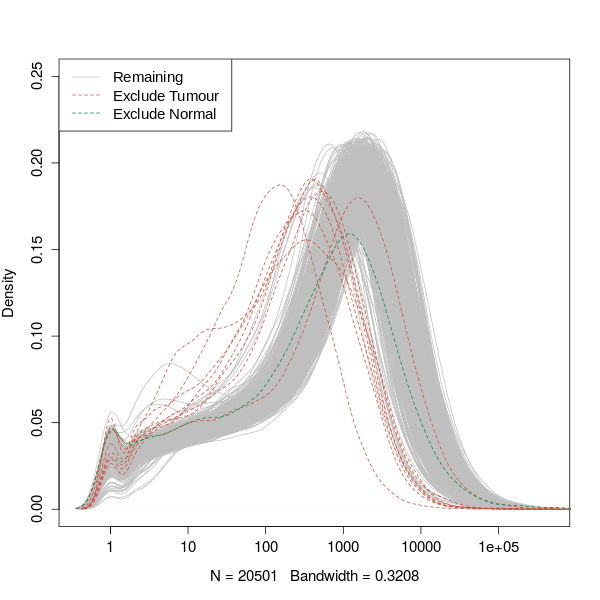
\includegraphics[width=0.4\textwidth]{fig2a.png}
        }%
        \subcaptionbox{Voom normalised}{%
           \label{fig:density:second}
           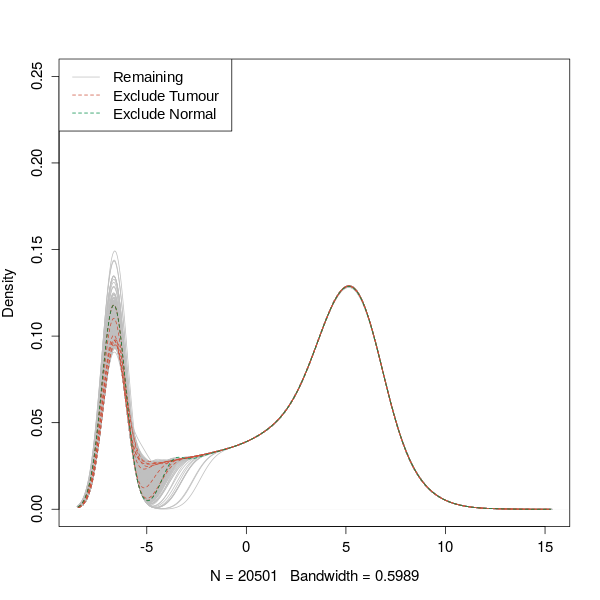
\includegraphics[width=0.4\textwidth]{fig2b.png}
        }%
%
\end{center}
\caption[Read count density]{\small \textbf{Read count density.} Sample density plots of raw counts on log-scale and voom normalised showing samples removed due to quality concerns.}
%}
\label{fig:density}
%\end{mdframed}
%\end{figure*}

%\begin{figure*}[!ht]
%\begin{mdframed}
%  \resizebox{\textwidth}{!}{
         \begin{center}
%
        \subcaptionbox{Mean raw counts (log-scale)}{%
            \label{fig:mean:first}
            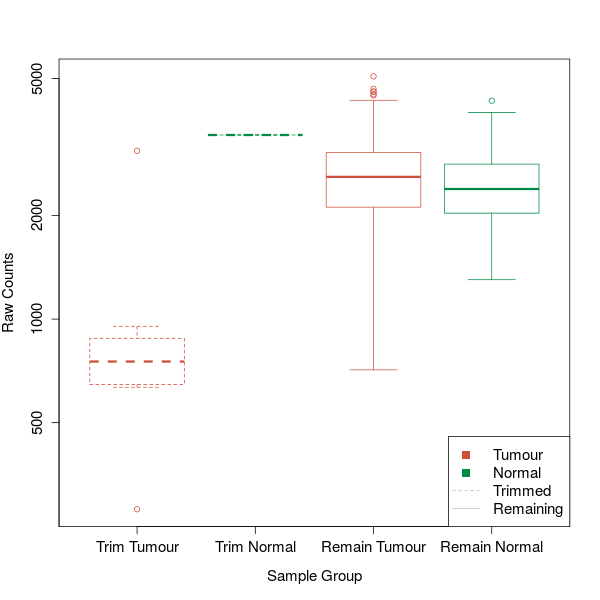
\includegraphics[width=0.4\textwidth]{fig3a.png}
        }%
        \subcaptionbox{Mean voom normalised}{%
           \label{fig:mean:second}
           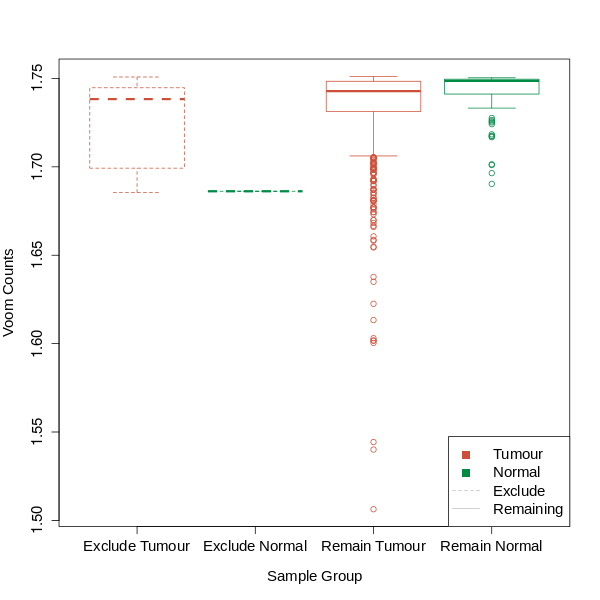
\includegraphics[width=0.4\textwidth]{fig3b.png}
        }%
%
    \end{center}
  \caption[Read count sample mean]{\small \textbf{Read count sample mean.} Boxplots of sample means for raw counts on log-scale and voom normalised show removed tumour samples with low mean read count.}
%}
\label{fig:boxplot}
%\end{mdframed}
\end{figure*}


\begin{table*}[!ht]
\caption{Excluded Samples by Batch and Clinical Characteristics.}
\label{tab:qc}
\resizebox{\textwidth}{!}{
      \begin{tabular}{sc^c^c^c^c^c^c^c^c^c^c^c^c}
      \rowstyle{\bfseries}
        \multicolumn{1}{c}{\bfseries Tissue Source}		& \multicolumn{1}{sc}{\bfseries Type}   & \multicolumn{1}{sc}{\bfseries Batch} & \multicolumn{1}{sc}{\bfseries Plate} & \multicolumn{1}{sc}{\bfseries Patient} & \multicolumn{1}{sc}{\bfseries Samples} & \multicolumn{1}{c}{\bfseries p53}      & \multicolumn{1}{sc}{\bfseries Subtype}   & \multicolumn{2}{sc}{\bfseries Treatment (History)}	& \multicolumn{3}{sc}{\bfseries Clinical Subtypes (Stage)} \\
        \hline
       \rowcolor{black!10}
        A7 Christiana		& Tumour & 47	 & A227  & A0DB  &  1 of 3   & NA       & Luminal A & Mastectomy & (no)					& ER$+$  &  Ductal   	& (2)        \\
       \rowcolor{black!5}
        A7 Christiana		& Tumour & 96	 & A220  & A13D  &  1 of 3   & Wildtype & Luminal A & Mastectomy & (no)					& ER$+$  &  Ductal   	& (2)        \\
       \rowcolor{black!10}
        A7 Christiana		& Tumour & 96	 & A227  & A13E  &  1 of 3   & NA       & Basal     & Lumpectomy & (no) 				& ER$-$  &  Ductal   	& (2)        \\
       \rowcolor{black!5}
        A7 Christiana		& Tumour & 142	 & A277  & A26E  &  1 of 3   & NA       & Basal     & Lumpectomy & (no) 				& ER$+$  &  Ductal   	& (2)        \\
       \rowcolor{black!10}
        A7 Christiana		& Tumour & 47	 & A277  & A0DC  &  1 of 2   & NA       & Luminal A & Mastectomy & (yes)				& ER$+$  &  Lobular   	& (3)        \\
       \rowcolor{black!5}
        A7 Christiana		& Tumour & 142	 & A220  & A26I  &  1 of 2   & Mutant   & Basal     & Lumpectomy & (yes) 				& ER$-$  &  Ductal   	& (2)        \\
       \rowcolor{black!10}
        AC Intl Genomics	& Tumour & 177	 & A18M  & A2QH  &  2 of 2   & Mutant   & Basal     & Radical Mastectomy & (no) 			& ER$-$  &  Metaplastic & (2)        \\
       \rowcolor{black!5}
        AC Intl Genomics	& Tumour & 177	 & A220  & A2QH  &  2 of 2   & Mutant   & Basal     & Radical Mastectomy & (no) 			& ER$-$  &  Metaplastic & (2)        \\
       \rowcolor{black!10}
        GI ABS IUPUI		& Normal & 177	 & A16F  & A2C8  &  1 of 1   & NA       & Luminal A & Radical Mastectomy and Neoadjuvant & (no) 	& ER$+$  &  Ductal   	& (2)        \\
\hline
      \end{tabular}
}
\end{table*}

Similarly, a correlation matrix of log-transformed raw counts was used to evaluate sample quality for \gls{TCGA} stomach RNASeq. A tumour sample (patient 4294) was removed due to similar quality concerns leaving a final dataset for 449 samples (from 417 patients): 414 tumour samples and 35 normal tissue samples.

\subsection{Metagenes and the Singular Value Decomposition} \label{methods:metagene}
A ``metagene'' offers a consistent signal of pathway (expression) activation or inactivation by dimension reduction of a matrix, avoiding negatively correlated genes averaging out the signal of a mean-based centroid \citep{Huang2003}. Constructing these pathway metagenes used gene sets for Reactome and Gatza signatures \citep{Gatza2011, Gatza2014} as specified above (see Section~\ref{methods:gene_set}). The singular-value decomposition was performed ($X = U^{T} D V$ where $X$ is the data matrix of the gene set with genes $\times$ samples) and the leading eigenvector (first column of $V$) corresponding to the largest singular value was used as a metagene for the pathway gene set. To ensure consistent directionality of metagene signals, the median of the gene set in each sample was calculated and correlated against the metagene with the (arbitrary) metagene sign adjusted as needed to conform with the majority of the gene set (i.e., positive correlation between metagene and the median-based centroid). To ensure that genes and pathways were weighted equally, metagenes were derived from a z-transformed dataset of gene expression and samples were scaled (by fractional ranking) for each metagene so that they were comparable on a $[0,1]$ scale. 

\subsubsection{Candidate Triage and Integration with Screen Data} \label{methods:venn_analysis}
Candidate triage in combination with the experimental data was intended to integrate findings of the \gls{SLIPT} analysis with an ongoing experiment project \citep{Chen2014, Telford2015}. The first procedure to compare the \gls{SLIPT} gene candidates for \textit{CDH1} with an \gls{siRNA} experimental screen \citep{Telford2015} was a direct comparison of the overlapping candidates, presented in a Venn diagram and tested with the $\chi^2$ test. Since these candidates modestly overlapped at the gene level (even when excluding genes not contained in both datasets), further gene set over-representation analysis was performed for pathways specific to each detection approach and the intersection of the two.

The pathway composition of the intersection was further verified by a permutation resampling analysis (as described in Section~\ref{methods:permutation}): the same number of genes detected by \gls{SLIPT} were sampled randomly from the universe of genes tested by both approaches. These samplings were performed over 1 million iterations and the pathway over-representation was compared for each of the 1652 reactome pathways.
%Adjusting for multiple comparisons was not needed here in a permutation analysis as the test $\chi^2$ statistics were directly used with the same degrees of freedom between expected and observed.
These over-representation scores ($\chi^2$) were compared the observed over-representation in the intersection of the \gls{SLIPT} candidates, with the proportion of resamplings with higher $\chi^2$ values used for empirical p-values of pathway composition. The $\chi^2$ test was used as an appropriation of Fisher's exact test on a hypergeometric distribution for resampling to computationally scale pathway over-representation tests across iterations.  Pathways for which no resamplings were occurred as high as the observed were reported as $p < 10^{-6}$. These empirical p-values were adjusted for multiple comparisons (FDR). Intersection size was not assumed to be constant across resamplings so similarly with the proportion of resamplings with higher or lower intersection size were used to evaluate significance of enrichment or depletion respectively (of \gls{siRNA} candidate among \gls{SLIPT} candidate genes).  

\section{Techniques}
Various statistical, computational, and bioinformatics techniques were performed throughout this thesis. This section describes these techniques and gives the parameters used unless otherwise specified. Where relevant, the R package implementation which provided the technique will be acknowledged. 

\subsection{Statistical Procedures and Tests}

As described in sections~\ref{methods:heatmap} and~\ref{methods:metagene}, the z-transform has been used to generate z-scores in various analyses in this thesis. Each row of dataset ($x$) is transformed into a scores ($z$) using the mean ($\mu$) and standard deviation ($\sigma$) of the data such that: $$ z = \frac{x - \mu(x)}{\sigma(x)} $$
This generates data where each row (gene) has a mean of 0 and standard deviation of 1. Where plotted as aa heatmap, any data more than 3 standard deviations above or below the mean is plotted as $3$ or $-3$ respectively.

Empirical Bayes differential expression analysis was performed using the \texttt{limma} R package \citep{limma}. Where specified, the Fisher's exact test, $\chi^2$ test, and correlation were used to measure associations between variables (as implemented in the \texttt{stats} R package \citep{R_core}). Unless otherwise specified, Pearson correlation was used for correlation analyses ($r$) and coefficient of determination ($R^2$). Where these comparisons are discussed in more detail, Fisher's exact test and $\chi^2$ tests are supported by a table or Venn diagram, rendered with the \texttt{limma} R package \citep{limma}. In some analyses, correlation is furter supported by a scatter plot and a line of best fit dervied by least squares linear regression. 

The \texttt{t.test} function \citep{R_core} has also been used to implement the t-test to compare pairs of data. Where relevant, an \gls{ANOVA} has been performed to report significance of multivariate predictors of outcomes, or least squares linear regression performed for the adjusted coefficient of determination ($R^2$) and F-statistic p-value to evaluate the fit of the predictor variables. For some analyses these are supported by boxplot or violinplot visualisation (rendered in R).

Multiple comparisons are adjusted by the Benjamini-Hochberg procedure to control the false discovery rate (FDR) unless otherwise specified \citep{fdr1995}. This procedure adjusts p-values to achieve an average of the proportion of false-positives among significant tests below a threshold, $\alpha$. The more stringent Holm-Bonferroni (Holm) procedure \citep{Holm1979} was also applied in some cases to adjust for multiple comparisons and control the family-wise error rate which adjusts p-values so that the probability that any one of the tests is a false-positive (type-1 error) below a threshold, $\alpha$.

\subsection{Gene Set Over-representation Analysis} \label{methods:enrichment}
Gene set enrichment over-representation was performed to test whether there is an enrichment of a gene set (e.g., a biological pathway) among a group of input genes. Such input genes may be predicted synthetic lethal candidates or a subset defined by clustering (in Section~\ref{methods:clustering}) or comparison with experimental candidates (see Section~\ref{methods:venn_analysis}). Initially, these tests were performed using the GeneSetDB web tool \citep{genesetdb} hosted by the University of Auckland on the Reactome pathways \citep{Reactome}. Since the GeneSetDB tool used an older version of Reactome (version 40), it was difficult to directly compare with the results of other analysis (see sections~\ref{methods:venn_analysis} and~\ref{methods:permutation}) performed on version 52 (as described in  Section~\ref{methods:gene_set}). Thus an implementation of the hypergeometric test in R \citep{R_core} was used to test for over-representation against Reactome (version 52) pathways. Pathways containing less than 10 genes or more than 500 \citep[as performed in GeneSetDB by][]{genesetdb} were excluded before adjusting for multiple comparisons.

\subsection{Clustering} \label{methods:clustering}
Clustering analysis when performed uses unsupervised hierarchical clustering with complete linkage (distance calculated from the furthest possible pairing). For correlation matrices or multivariate normal parameters (e.g., $\Sigma$), the distance metric used was Euclidean distance. For empirical or simulated gene and pathway expression data correlation distance was used, calculated by $distance = 1 - cor(t(x))$ where $cor$ is Pearson correlation and $t(x)$ is the transpose of the expression matrix. 

\subsection{Heatmap} \label{methods:heatmap}
Standardised z-scores of the data were used to plot heatmaps on an appropriate scale. Raw (log-scale) read counts or voom normalised counts per gene (as specified) were plotted  as normalised z-scores on a $[-3,+3]$ blue-red scale. Similarly, correlations were plotted on a $[-1,+1]$ blue-red scale. These heatmaps were performed using the linkage and distance specified for the clustering performed in Section~\ref{methods:clustering}. The \texttt{gplots} R package \citep{gplots} was used to generate many of the heatmaps throughout this thesis, along with a customised heatmap function (released as \texttt{heatmap.2x}). Where clearly specified, data have been split into subsets with clustering performed separately on each subset with these plotted alongside each other.

\subsection{Modeling and Simulations} \label{methods:simulation}
Statistical modeling and simulations have been used to test various synthetic lethal detection procedures on simulated data. This involves constructing a statistical model of how synthetic lethality would appear in (continuous normally distributed) gene expression data. Where presented (in Section~\ref{methods:SL_Model}), the assumptions of the model are stated clearly. The model allows sampling from a multivariate normal distribution (using the \texttt{mvtnorm} R package \citep{Genz2009, mvtnorm}) to generate simulated data with known underlying synthetic lethal partners (detailed in Section~\ref{methods:simulating_SL}). We can test whether statistical procedures, including those developed in this thesis (presented in Section~\ref{methods:SLIPT}), are capable of detecting them upon this simulated data. This multivariate normal simulation procedure also enables the inclusion of correlation structure which is either given as correlated blocks of genes or derived from pathway structures (as detailed in Section~\ref{methods:graphsim}).

If this multivariate normal distribution was sampled once and the procedure to add known synthetic lethal partners was performed, it generates a simulated dataset. Performing this simulation procedure and testing with a synthetic lethal detection procedure iteratively, these simulations can be used to assess the statistical performance of the detection procedure. The number of iterations (\texttt{Reps}) will be given for each simulation result. Typically, these are performed 1000 or 10,000 times depending on computational feasibility of doing so on larger datasets. 

Several measures of statistical performance were used to assess the simulations. The following measures used the final classification of the detection procedure, statistical significance for $\chi^2$, significance and directional criteria met for \gls{SLIPT} (see Section~\ref{methods:SLIPT}), and an arbitrary threshold: $<-0.2$ and $>+0.2$ for  negative correlation and correlation respectively. Sensitivity (or ``true positive rate'') was measured as the proportion of known synthetic lethal partners predicted to be synthetic lethal. Specificity (or ``true negative rate'') was measured as the proportion of known non-synthetic lethal partners predicted not to be synthetic lethal. The ``false discovery rate'' (also used in adjusting for multiple comparisons) was measured here as the proportion of known non-synthetic lethal partners out of all putative partners predicted by the detection procedure. Statistical ``accuracy'' is the proportion of true predictions for a detection procedure, which is both the correctly predicted known synthetic lethal partners and correctly negative known non-synthetic lethal partners.

\subsubsection{Receiver Operating Characteristic (Performance)}
A more general procedure to measure the statistical performance of a simulation is the Receiver Operating Characteristic (ROC) curve which does not assume a threshold for classification of synthetic lethality but demonstrates the trade-off of sensitivity and specificity \citep{Zweig1993, Fawcett2006, Akobeng2007}. These curves (implemented with the \texttt{ROCR} R package \citep{ROCR}) plot the True Positive Rate (sensitivity) against the False Positive Rate ($1-$specificity) as the prediction threshold is varied. An ideal detection method will have a true positive rate of 1 and a false positive rate of 0, hence the Area Under the ROC curve (AUC or AUROC) is a measure of statistical performance for a detection procedure accounting for this trade-off. AUROC values are typically range from 0.5 the value expected by random chance to 1 for an optimal detection method, however it is possible for an AUROC below 0.5 for a poor detection method that performs worse than random chance. An cancer biology, an AUROC of approximately $0.8$ is a predictive biomarker suitable for publication \citep{Hajian-Tilaki2013} but predictors with lower AUROC values may still be informative depending on the context. In this thesis, the AUROC values varies widely across simulation parameters and a primarily used for comparisons across these parameters, although they can also be used to refine thresholds for optimal classification. 

\subsection{Resampling Analysis} \label{methods:permutation}
Resampling analyses (e.g., ``permutation'' analysis) are used to statistically test the significance of an observation without assuming the underlying distribution of expected test statistics \citet{Collingridge2013}. Instead these are derived from randomly shuffling test statistics or randomly sampling predicted candidates. For the purposes of this thesis, this involved randomly sampling genes from those tested to be analysed as putative synthetic lethal candidates. This was performed both for testing the significance of pathway composition in the intersection with experimental gene candidates (Section~\ref{methods:venn_analysis}) and for assessing the significance of pathway structure among synthetic lethal candidates (Section~\ref{methods:network_permutation}).

These were analysed to compare the observed synthetic lethal genes against values derived from randomly sampling the same number of genes as observed by synthetic lethal from among the genes tested. Sampling iteratively across many resampling procedures, these resampling-based values form a null distribution that would be observed if the null hypothesis were true. Thus the proportion of resampling-based values across these iterations that are greater than or equal to that observed, forms an empirically derived p-value to test significance.

Resampling was performed for comparison (in Section~\ref{methods:venn_analysis}) with fixed experimental screen candidates \citep{Telford2015} both resampling the number of genes overlapping with the screen candidates and test statistics for pathway enrichment. Resampling analysis was also applied to shortest paths and network metrics (in Section~\ref{methods:network_permutation}) to test significance of directional relationships between synthetic lethal candidate genes within pathway structures.

The number of iterations determines the accuracy of these p-values. For pathway composition (in Section~\ref{methods:venn_analysis}), a million iterations were performed using high performance computing (as detailed in Section~\ref{methods:HPC}) to provide sufficient accuracy after adjusting for multiple comparisons across pathways. For the purposes of network analysis (in Section~\ref{methods:network_permutation}), a thousand iterations were sufficient to reject the null hypothesis for the majority of pathways tested before adjusting for multiple comparisons, and thus further iterations were not performed.

\section{Pathway Structure Methods}

\subsection{Network and Graph Analysis}

Networks are important in considering the structure of relationships in molecular biology, including gene regulation, kinase cellular signalling, and metabolic pathways \citep{Barabasi2004}. Network theory is an interdisciplinary field which combines the approaches of computer science with the metrics and fundamental principles of graph theory, an area of pure mathematics dealing with relationships between sets of discrete elements. The vast amounts of molecular and cellular data from high-throughput technologies have enabled the application of network-based and genome-wide bioinformatics analysis to examine the complexity of a cell at the molecular level and understand aberrations in cancer. This thesis uses various metrics and analysis procedures developed in Graph and Network theory to analyse graph structure of biological pathways. Where feasible, these have been implemented using the \texttt{igraph} R package with such procedures described below \citep{igraph}. Custom R functions to perform more complex analysis and visualisation of iGraph data objects will be described later.

Graph theory is a branch of pure mathematics which deals with the properties of sets of discrete objects (referred to as a `node' or `vertex`) with some pairs are joined (by a `link' or an `edge`). While a seemingly reductionist abstraction to mathematically study relationships, graph theory serves has applications in a wide range of studies including life sciences. Network theory is the sub-discipline of graph theory which deals with networks which has become popular due to the vast potential for applications of networks \citep{vanSteen2010}. 

Applications vary depending on the situation modelled, particularly in how the edges between vertices are defined, whether they are directed or weighted, and whether multiple redundant edges between a pair of vertices (referred to as `parallel edges`) or edges connecting a vertex to itself (referred to as `loops`) are permitted in the model. Networks are defined such that the edges represent a relationship between the vertices and may be directed, weighted, or contain parallel edges or loops depending on the application \citep{vanSteen2010}. Unless otherwise stated, graph structures and networks in thesis will be unweighted and have no parallel edges or loops. Where a directional relationship is known or modelled, it will be represented with a directed edge in a directed graph.

\subsection{Sourcing Graph Structure Data} \label{methods:graph_data}
Pathway Commons interaction data was sourced using \gls{BioPAX} with the paxtools-4.3.0 Java application on October 6\textsuperscript{th} 2015 \citep{PathwayCommons, paxtools}. This utility was used to source `sif' format interaction data into R \citep{R_core}, from which the human Reactome (version 52) dataset of interactions was imported \citep{Reactome}, matching those used for pathway enrichment analysis. These interactions were used to construct an adjacency matrix for the Reactome network and subnetworks corresponding to each relevant biological pathway. 

\subsection{Constructing Pathway Subgraphs} \label{methods:subgraphs}
Subgraphs for each relevant pathway were constructed by matching the nodes in the complete Reactome network to the pathway gene sets (as derived in Section~\ref{methods:gene_set}). A subgraph with adjacent nodes was constructed by adding nodes which have an edge with a gene in the pathway gene set. The pathways these adjacent nodes belong to were added to form a ``meta-pathway'' to account for the possibility for nodes within the pathway being linked by the surrounding graph structure.

\subsection{Network Analysis Metrics} \label{methods:network_metrics}
The existing network analysis measures applied in this thesis (as described below) used an implementation in the \texttt{igraph} R package where it was available \citep{igraph}. Otherwise, custom features were developed for analysis of iGraph objects in R and released as \texttt{igraph.extensions} (as described in Section~\ref{methods:igraph_extensions}).

Vertex degree is the number of edges a node has and is a fundamental measure of the importance and connectivity of a network \citep{vanSteen2010}. More connected nodes, such as network hubs, will have a higher vertex degree relative to other nodes. For the purposes of this thesis, vertex degree ignored edge direction with loops (edges with itself) and double edges to the same node excluded.

A fundamental concept in network analysis is a ``shortest path'', that is the shortest route via edges between any two particular nodes in a network. These are computed by Dijstra's algorithm \citep{Dijkstra1959} in the \texttt{igraph} R package \citep{igraph}. Where applicable paths will only use directed edges in a particular direction. Shortests paths are a useful measure of how close nodes are in a network. This is used to compute information centrality, and for further analysis of pathway structure (as described in Section~\ref{methods:pathway_str}).

Network centrality is an alternative measure of the importance or influence of a node to the graph structure \citep{Borgatti2005}. Various strategies are used to derive centrality,  typically based on how connected the node is or the impact of node removal on the connectivity of the network. One of the most notable is the ``PageRank'' algorithm, a refinement of eigenvector centrality based on the eigenvectors of the adjacency matrix \citep{Brin1998}. This is implemented in the \texttt{igraph} R package \citep{igraph}.

Another network centrality measure that has been previously applied to biological protein interaction networks \citep{Kranthi2013} is the ``information centrality''. The information centrality of a node is the relative impact on efficiency (transmission of information via shortest paths) of the network when the node is removed. That is the centrality ($C$) \citep{Kranthi2013} for node $n$ in graph $G$ is defined as: $$C_n = \frac{E(G)-E(G')}{E(G)}$$ where $G'$ is the subgraph with the node removed and $E$ is the efficiency \citep{Latora2001} derived from shortest paths ($d_{ij}$ between nodes $i$ and $j$) as: $$E(G) = \frac{2}{N(N-1} \sum_{i<j \in G}^{} \frac{1}{d_{ij}}$$ The efficiency of the network can be derived from shortest paths implemented in the \texttt{igraph} R package and the iterative network centrality computation of each node has been released as an R package (\texttt{info.centrality}) and included in the \texttt{igraph.extensions} package.

\section{Implementation}
%\subsection{Computational Tools and Enabling Biological Research (remove/state assumptions only)}
%\subsubsection{Computational Tools for Biological Research}
%In addition to hosting data repositories on the web, tools developed with computational expertise have had wider benefit in  genetics research. One of the main impacts of a techniques developed from computer science is the alignment of reads, to either assemble a genome \textit{de novo} from it's reads or map reads to a pre-existing reference genome. Mapping reads is commonplace to call variants between samples, this is useful for studies of human disease interested in risks of these variants or wider application such as comparing populations or species in an evolution phylogeny. Mapping reads has further utility in functional genetics to identify which regions or a genome are expressed or have DNA methylation. Similarly, mapping is used to map RNA-Seq or Bisulfite-Seq reads to measure gene expression or DNA methylation across the genome in a cohort or sample. While mapping is not performed in this thesis, it has performed an important role in the adoption of genomics in genetics research.



\subsection{Computational Resources and Linux Utilities}

Several computers were used to process and store data during this thesis (as summarised in Table~\ref{tab:computers}), running different versions of Linux operating systems, including a personal laptop computer, laboratory desktop machine, departmental server, and the New Zealand eScience Infrastructure Intel Pan high-performance computing cluster (a supercomputer based at the University of Auckland). Each of these systems support a 64-bit architecture. Current workflows on local machines use Elementary OS (based on the Ubuntu versions given in Table~\ref{tab:computers}) and interacting with these via ZSH shell. However, Ubuntu OS and the Bourne Again SHell (bash) were used at the inception of this project and bash is continues to be used for running scripts. Various Linux applications and command-line utilities were used on these machines (as summarised in Table~\ref{tab:computers_linux}). As such, the workflows developed in this project should be backwards-compatible with Ubuntu Linux (and other derivatives). The majority of novel methodology and implementations were performed in R which is a cross-platform language, packages developed in R will be available for users of Linux, Mac, and Windows machines.  


\begin{table}[!ht]
\centering
\caption{Computers used during Thesis}
\label{tab:computers}
\makebox[\textwidth][c]{
\resizebox{\textwidth}{!}{
\begin{tabular}{r|l|l|l|l|}
%\cline{2-5}
\multicolumn{1}{r}{}                        & \multicolumn{1}{l}{\bfseries Viao Laptop}                                     & \multicolumn{1}{l}{\bfseries Lab Machine}                                   & \multicolumn{1}{l}{\bfseries Biochem Server}                                     & \multicolumn{1}{l}{\bfseries NeSI Pan Cluster}                               \\
\cline{2-5}
\rowcolor{black!10}
\multicolumn{1}{r|}{\cellcolor{white}Operating System (OS)}  & \begin{tabular}[c]{@{}l@{}}Elementary OS\\ Freya 0.3.2\end{tabular} & \begin{tabular}[c]{@{}l@{}}Elementary OS\\ Loki 0.4\end{tabular}  & \begin{tabular}[c]{@{}l@{}}Red Hat Enterprise\\ Maipo 7.2\end{tabular} & \begin{tabular}[c]{@{}l@{}}Cent OS\\ Final 6.4\end{tabular} \\ 
%\cline{2-5}
\rowcolor{black!5}
\multicolumn{1}{r|}{\cellcolor{white}Upstream OS}            & \begin{tabular}[c]{@{}l@{}}Ubuntu LTS\\ Trusty 14.04\end{tabular}   & \begin{tabular}[c]{@{}l@{}}Ubuntu LTS\\ Xenial 16.04\end{tabular} &                                                                        &                                                             \\ 
%\cline{2-5}
\rowcolor{black!10}
\multicolumn{1}{r|}{\cellcolor{white}Linux Kernel}           & 3.19.0-65-generic                                                   & 4.4.0-36-generic                                                  & 3.10.0-327.36.2.el7.x86\_64                                            & 2.6.32-504.16.2.el6.x86\_64                    \\
%\cline{2-5}
\rowcolor{black!5}
\multicolumn{1}{r|}{\cellcolor{white}Shell: bash}            & 4.3.11(1)                                                           & 4.3.46(1)                                                         & 4.2.46(1)                                                              & 4.2.1(1)                                       \\
%\cline{2-5}
\rowcolor{black!10}
\multicolumn{1}{r|}{\cellcolor{white}Shell: zsh}             & 5.0.2                                                               & 5.1.1                                                             & 5.0.2                                                                  & 5.2                                            \\
\cline{2-5}
\end{tabular}
}}
\end{table}


\begin{table}[!ht]
\centering
\caption{Linux Utilities and Applications used during Thesis}
\label{tab:computers_linux}

\resizebox{\textwidth}{!}{
\begin{tabular}{|ll|l|l|l|l|}
%\cline{3-6}
\multicolumn{1}{l}{\cellcolor{white}}                                 & \multicolumn{1}{l}{}                         & \multicolumn{1}{l}{\bfseries Viao Laptop}                           & \multicolumn{1}{l}{\bfseries Lab Machine}                         & \multicolumn{1}{l}{\bfseries Biochem Server}                           & \multicolumn{1}{l}{\bfseries NeSI Pan Cluster}                               \\
\cline{2-6}
\rowcolor{black!10}
\multicolumn{1}{l}{\cellcolor{white}}                                 & \multicolumn{1}{|l|}{OS}                     & \begin{tabular}[c]{@{}l@{}}Elementary OS\\ Freya 0.3.2\end{tabular} & \begin{tabular}[c]{@{}l@{}}Elementary OS\\ Loki 0.4\end{tabular}  & \begin{tabular}[c]{@{}l@{}}Red Hat Enterprise\\ Maipo 7.2\end{tabular} & \begin{tabular}[c]{@{}l@{}}Cent OS\\ Final 6.4\end{tabular} \\
%\cline{2-6}
\rowcolor{black!5}
\multicolumn{1}{l}{\cellcolor{white}}                                 & \multicolumn{1}{|l|}{Linux Kernel}           & 3.19.0-65-generic                                                   & 4.4.0-36-generic                                                  & 3.10.0-327.36.2.el7.x86\_64                                            & 2.6.32-504.16.2.el6.x86\_64                    \\
\hline
\rowcolor{black!10}
\cellcolor{white} Scripting                                            & \multicolumn{1}{|l|}{Shell\: bash}            & 4.3.11(1)                                                           & 4.3.46(1)                                                         & 4.2.46(1)                                                              & 4.2.1(1)                                       \\
%\cline{2-6}
\rowcolor{black!5}
\cellcolor{white}                                                      & \multicolumn{1}{|l|}{Shell\: zsh}             & 5.0.2                                                               & 5.1.1                                                             & 5.0.2                                                                  & 5.2                                            \\
\hline
\rowcolor{black!10}
\cellcolor{white} Programming                                          & \multicolumn{1}{|l|}{Python}                 & 2.7.6                                                               & 2.7.12                                                            & 2.7.5                                                                  &                                                \\
%\cline{2-6}
\rowcolor{black!5}
\cellcolor{white}                                                      & \multicolumn{1}{|l|}{Java}                   & 1.8.0\_101                                                          & 9-ea                                                              & 1.8.0\_101                                                             &                                                \\
%\cline{2-6}
\rowcolor{black!10}
\cellcolor{white}                                                      & \multicolumn{1}{|l|}{C$++$}                  & 4.8.4                                                               & 5.4.0                                                             & 4.8.5                                                                  & 4.4.7                                          \\
\hline
\rowcolor{black!5}
\cellcolor{white} Text Editor                                          & \multicolumn{1}{|l|}{nano}                   & 2.2.6                                                               & 2.5.3                                                             & 2.3.1                                                                  & 2.0.9                                          \\
%\cline{2-6}
\rowcolor{black!10}
\cellcolor{white}                                                      & \multicolumn{1}{|l|}{kile (\LaTeX)}          & 2.1.3                                                               & 2.1.3                                                             &                                                                        &                                                \\
\hline
\rowcolor{black!5}
\cellcolor{white} Version Control                                      & \multicolumn{1}{|l|}{git}                    & 1.9.1                                                               & 2.11.0                                                            & 1.7.1                                                                  & 1.8.3.1                                        \\
\hline
\rowcolor{black!10}
\cellcolor{white} Shell Utilities                                      & \multicolumn{1}{|l|}{sed}                    & 4.4.2                                                               & 4.4.2                                                             & 4.4.2                                                                  & 4.4.1                                          \\
%\cline{2-6}
\rowcolor{black!5}
\cellcolor{white}                                                      & \multicolumn{1}{|l|}{grep}                   & 2.16-1                                                              & 2.25-1                                                            & 2.20                                                                   & 2.6.3                                          \\
%\cline{2-6}
\rowcolor{black!10}
\cellcolor{white}                                                      & \multicolumn{1}{|l|}{nohup}                  & 8.21                                                                & 8.25                                                              & 8.22                                                                   & 8.4                                            \\
\hline
\rowcolor{black!5}
\cellcolor{white} Typesetting                                          & \multicolumn{1}{|l|}{\TeX}                   & 3.1415926                                                           & 3.14159265                                                        &                                                                        &                                                \\
%\cline{2-6}
\rowcolor{black!10}
\cellcolor{white}                                                      & \multicolumn{1}{|l|}{TexLive (\LaTeX)}       & 2013                                                                & 2015                                                              &                                                                        &                                                \\
%\cline{2-6}
\rowcolor{black!5}
\cellcolor{white}                                                      & \multicolumn{1}{|l|}{PDF\TeX}                & 2.5-1                                                               & 2.6                                                               &                                                                        &                                                \\
%\cline{2-6}
\rowcolor{black!10}
\cellcolor{white}                                                      & \multicolumn{1}{|l|}{pandoc}                 & 1.12.2.1                                                            & 1.16.0.2                                                          &                                                                        &                                                \\
\hline
\rowcolor{black!5}
\cellcolor{white} Remote Computing                                     & \multicolumn{1}{|l|}{Slurm scheduler}        &                                                                     &                                                                   &                                                                        & 16.05.6                                        \\
%\cline{2-6}
\rowcolor{black!10}
\cellcolor{white}                                                      & \multicolumn{1}{|l|}{OpenSSH}                & 7.2p2                                                               & 7.2p2                                                             & 6.6.1                                                                  & 5.3p1                                          \\
%\cline{2-6}
\rowcolor{black!5}
\cellcolor{white}                                                      & \multicolumn{1}{|l|}{OpenSSL}                & 1.0.2g                                                              & 1.0.2g                                                            & 1.0.01e-fips                                                           & 1.0.01e-fips                                   \\
%\cline{2-6}
\rowcolor{black!10}
\cellcolor{white}                                                      & \multicolumn{1}{|l|}{rsync}                  & 3.1.0p31                                                            & 3.1.1p31                                                          & 3.0.9p30                                                               &                                                \\
%\cline{2-6}
\rowcolor{black!5}
\cellcolor{white}                                                      & \multicolumn{1}{|l|}{Globus Online Transfer} &                                                                     &                                                                   & 3.1                                                                    & 3.1                                            \\
%\cline{2-6}
\rowcolor{black!10}
\cellcolor{white}                                                      & \multicolumn{1}{|l|}{Cisco AnyConnect VPN}   &                                                                     & 3.1.05170                                                         &                                                                        &                                                \\
\hline
\rowcolor{black!5}
\cellcolor{white} Image Processing                                     & \multicolumn{1}{|l|}{Inkscape}               & 0.48.4                                                              & 0.91                                                              &                                                                        &                                                \\
%\cline{2-6}
\rowcolor{black!10}
\cellcolor{white}                                                      & \multicolumn{1}{|l|}{GIMP}                   & 2.8.10                                                              & 2.8.16                                                            &                                                                        &                                                \\
%\cline{2-6}
\rowcolor{black!5}
\cellcolor{white}                                                      & \multicolumn{1}{|l|}{ImageMagick}            & 6.7.7.10-6                                                          &                                                                   &                                                                        &                                                \\
\hline                                
\end{tabular}
}
\end{table}


\FloatBarrier

\subsection{R Language and Packages}


The R programming language has been used for the majority of this thesis. Current R installations across the machines used are given in Table~\ref{tab:computers_r}. Local machines currently run the latest version of the R (at the time of writing) and remote machines run the versions and modules as managed by the system administrator.

Various scripts and packages in this thesis were developed or run in previous versions of RStudio and R but these run without error in the current version of R (and the older versions on remote machines). The R packages which were used throughout this thesis (as detailed in Table~\ref{tab:computers_r_packages} with versions specified) were installed from the Comprehensive R Archive Network \citep{CRAN}, Bioconductor \citep[][version 3.4; BiocInstaller 1.24.0]{Gentleman2004}, or GitHub. These packages were not updated when they would change the functionality of scripts or functions in packages, in particular imported data from annotation packages (used to define gene sets) have been saved as local files to continue using stable versions of these pathway data (across machines).

This is a summary of the key packages which (in addition to their dependencies) have been used throughout this project. Where a package implementation has been central to the methods applied, they are described in more detail in the relevant section. A full table of packages used in this thesis can be found in Appendix~\ref{appendix:software} (Table~\ref{tab:computers_r_packages_full}). The R packages developed during this thesis are given in Table~\ref{tab:computers_r_packages_dev} with the relevant sections describing their implementation and use where appropriate, in addition to further details on these functions in Section~\ref{methods:r_packages}. 

\begin{table}[!ht]
\centering
\caption{R Installations used during Thesis}
\label{tab:computers_r}
\resizebox{\textwidth}{!}{
\begin{tabular}{|ll|l|l|l|l|}
%\cline{3-6}
\multicolumn{1}{l}{\cellcolor{white}}   & \multicolumn{1}{l}{}              & \multicolumn{1}{l}{\bfseries Viao Laptop}                           & \multicolumn{1}{l}{\bfseries Lab Machine}                         & \multicolumn{1}{l}{\bfseries Biochem Server}                           & \multicolumn{1}{l}{\bfseries NeSI Pan Cluster}           \\
\cline{2-6}
\rowcolor{black!10}
\multicolumn{1}{l}{\cellcolor{white}}   & \multicolumn{1}{|l|}{OS}          & \begin{tabular}[c]{@{}l@{}}Elementary OS\\ Freya 0.3.2\end{tabular} & \begin{tabular}[c]{@{}l@{}}Elementary OS\\ Loki 0.4\end{tabular}  & \begin{tabular}[c]{@{}l@{}}Red Hat Enterprise\\ Maipo 7.2\end{tabular} & \begin{tabular}[c]{@{}l@{}}Cent OS\\ Final 6.4\end{tabular} \\
\hline
\rowcolor{black!5}
\cellcolor{white} Programming           & \multicolumn{1}{|l|}{R}           & 3.3.2                                                               & 3.3.2                                                             & 3.3.1                                                                  & 3.3.0-intel (module)                          \\
\hline

\rowcolor{black!10}
\cellcolor{white} Development           & \multicolumn{1}{|l|}{RStudio}     & 1.0.136                                                             & 1.0.136                                                           & 1.0.136 (server)                                                       &                                                \\
\hline
\end{tabular}
}
\end{table}

%\resizebox{\textwidth}{!}{
\setlength{\LTleft}{-20cm plus -1fill}
\setlength{\LTright}{\LTleft}

\begin{longtable}{llll}
\caption{R Packages used during Thesis}
\label{tab:computers_r_packages}
%\\ hline
\\
\multicolumn{1}{l}{\bfseries Package}      & \multicolumn{1}{l}{\bfseries Version Used} & \multicolumn{1}{l}{\bfseries Built} & \multicolumn{1}{l}{\bfseries Repository}      \\
\hline  \rowcolor{black!10}
colorspace   & 1.3-2          & 3.3.1 & CRAN            \\
%\hline  
\rowcolor{black!5}
curl         & 2.3            & 3.3.1 & CRAN            \\
%\hline  
\rowcolor{black!10}
data.table   & 1.9.6          & 3.3.1 & CRAN            \\
%\hline  
\rowcolor{black!5}
dendextend   & 1.4.0          & 3.3.2 & CRAN            \\
%\hline  
\rowcolor{black!10}
DBI          & 0.5-1          & 3.3.1 & CRAN            \\
%\hline  
\rowcolor{black!5}
devtools     & 1.12.0         & 3.3.1 & CRAN            \\
%\hline  
\rowcolor{black!10}
dplyr        & 0.5.0          & 3.3.1 & CRAN            \\
%\hline  
\rowcolor{black!5}
ggplot2      & 2.2.1          & 3.3.1 & CRAN            \\
%\hline  
\rowcolor{black!10}
git2r        & 0.18.0         & 3.3.1 & CRAN            \\
%\hline  
\rowcolor{black!5}
gplots       & 3.0.1          & 3.3.1 & CRAN            \\
%\hline  
\rowcolor{black!10}
gtools       & 3.5.0          & 3.3.1 & CRAN            \\
%\hline  
\rowcolor{black!5}
igraph       & 1.0.1          & 3.3.1 & CRAN            \\
%\hline  
\rowcolor{black!10}
matrixcalc   & 1.0-3          & 3.3.1 & CRAN            \\
%\hline  
\rowcolor{black!5}
mclust       & 5.2.2          & 3.3.1 & CRAN            \\
%\hline  
\rowcolor{black!10}
mvtnorm      & 1.0-6          & 3.3.1 & CRAN            \\
%\hline  
\rowcolor{black!5}
org.Hs.eg.db & 3.1.2          & 3.1.2 & Bioconductor    \\
%\hline  
\rowcolor{black!10}
openssl      & 0.9.6          & 3.3.1 & CRAN            \\
%\hline  
\rowcolor{black!5}
plyr         & 1.8.4          & 3.3.1 & CRAN            \\
%\hline  
\rowcolor{black!10}
purrr        & 0.2.2          & 3.3.1 & CRAN            \\
%\hline  
\rowcolor{black!5}
reactome.db  & 1.52.1         & 3.2.1 & Bioconductor    \\
%\hline  
\rowcolor{black!10}
RColorBrewer & 1.1-2          & 3.3.1 & CRAN            \\
%\hline  
\rowcolor{black!5}
Rcpp         & 0.12.9         & 3.3.1 & CRAN            \\
%\hline  
\rowcolor{black!10}
ROCR         & 1.0-7          & 3.3.1 & CRAN            \\
%\hline  
\rowcolor{black!5}
roxygen2     & 6.0.1          & 3.3.2 & CRAN            \\
%\hline  
\rowcolor{black!10}
shiny        & 1.0.0          & 3.3.1 & CRAN            \\
%\hline  
\rowcolor{black!5}
snow         & 0.4-2          & 3.3.1 & CRAN            \\
%\hline  
\rowcolor{black!10}
testthat     & 1.0.2          & 3.3.2 & CRAN            \\
%\hline  
\rowcolor{black!5}
tidyr        & 0.6.1          & 3.3.2 & CRAN            \\
%\hline  
\rowcolor{black!10}
tidyverse    & 1.1.1          & 3.3.2 & GitHub (hadley) \\
%\hline  
\rowcolor{black!5}
sm           & 2.2-5.4        & 3.3.1 & CRAN            \\
%\hline  
\rowcolor{black!10}
Unicode      & 9.0.0-1        & 3.3.2 & CRAN            \\
%\hline  
\rowcolor{black!5}
vioplot      & 0.2            & 3.3.1 & CRAN            \\
%\hline  
\rowcolor{black!10}
viridis      & 0.3.4          & 3.3.2 & CRAN            \\
%\hline  
\rowcolor{black!5}
xml2         & 1.1.1          & 3.3.2 & CRAN            \\
%\hline  
\rowcolor{black!10}
xtable       & 1.8-2          & 3.3.1 & CRAN            \\
%\hline  
\rowcolor{black!5}
zoo          & 1.7-14         & 3.3.1 & CRAN            \\
%\hline  
\rowcolor{black!10}
graphics     & 3.3.2          & 3.3.2 & base            \\
%\hline  
\rowcolor{black!5}
grDevices    & 3.3.2          & 3.3.2 & base            \\
%\hline  
\rowcolor{black!10}
cluster      & 2.0.5          & 3.3.1 & base            \\
%\hline  
\rowcolor{black!5}
graphics     & 3.3.2          & 3.3.2 & base            \\
%\hline  
\rowcolor{black!10}
grDevices    & 3.3.2          & 3.3.2 & base            \\
%\hline  
\rowcolor{black!5}
Matrix       & 1.2-8          & 3.3.1 & base            \\
%\hline  
\rowcolor{black!10}
stats        & 3.3.2          & 3.3.2 & base            \\
\hline
\end{longtable}

\begin{table}[!ht]
\centering
\caption{R Packages Developed during Thesis}
\label{tab:computers_r_packages_dev}
\resizebox{\textwidth}{!}{
\begin{tabular}{|l|llc|}
%\cline{2-4}
\multicolumn{1}{l}{}           & \multicolumn{1}{l}{\bfseries Package Name} & \multicolumn{1}{l}{\bfseries Description                                                   and GitHub Repository}                                                                   & \multicolumn{1}{c}{\bfseries Section} \\
\cline{2-4}  \rowcolor{black!10}
\multicolumn{1}{l|}{\cellcolor{white}}           & \multicolumn{1}{l}{\texttt{slipt}}        & \begin{tabular}[c]{@{}l@{}}Synthetic lethal detection by \gls{SLIPT} (to accompany publication)  \\ \url{https://github.com/TomKellyGenetics/slipt}                         \end{tabular} & \ref{methods:SLIPT}  \\
\hline
\rowcolor{black!5} \cellcolor{white}
visualisation                  & \texttt{vioplotx}                          & \begin{tabular}[c]{@{}l@{}}Customised violin plots (based on \texttt{vioplot})             \\ \url{https://github.com/TomKellyGenetics/vioplotx}                      \end{tabular} &                              \\
%\cline{2-4}
\rowcolor{black!10} \cellcolor{white}
                               & \texttt{heatmap.2x}                      & \begin{tabular}[c]{@{}l@{}}Customised heatmaps (based on \texttt{gplots})                  \\ \url{https://github.com/TomKellyGenetics/heatmap.2x}                    \end{tabular} & \ref{methods:heatmap} \\
\hline
\rowcolor{black!5} \cellcolor{white}
\texttt{igraph.extensions}     & \texttt{igraph.extensions}               & \begin{tabular}[c]{@{}l@{}}Meta-package to install the follow iGraph functions             \\ \url{https://github.com/TomKellyGenetics/igraph.extensions}             \end{tabular} & \ref{methods:igraph_extensions}    \\
%\cline{2-4}

\rowcolor{black!10} \cellcolor{white}
                               & \texttt{plot.igraph}                     & \begin{tabular}[c]{@{}l@{}}Custom plotting of directed graphs                              \\ \url{https://github.com/TomKellyGenetics/plot.igraph}                   \end{tabular} & \ref{methods:network_metrics}      \\
%\cline{2-4}
\rowcolor{black!5} \cellcolor{white}
                               & \texttt{info.centrality}                 & \begin{tabular}[c]{@{}l@{}}Computing information centrality from network efficiency        \\ \url{https://github.com/TomKellyGenetics/info.centrality}               \end{tabular} & \ref{methods:graphsim}\\
%\cline{2-4}

\rowcolor{black!10} \cellcolor{white}
                               & \texttt{pathway.structure.permutation}   & \begin{tabular}[c]{@{}l@{}}Testing pathway structure with resampling analysis              \\ \url{https://github.com/TomKellyGenetics/pathway.structure.permutation} \end{tabular} & \ref{methods:network_permutation}  \\
%\cline{2-4}
\rowcolor{black!5} \cellcolor{white}
                               & \texttt{graphsim}                        & \begin{tabular}[c]{@{}l@{}}Generating simulated expression from graph structures           \\ \url{https://github.com/TomKellyGenetics/graphsim}                      \end{tabular} & \ref{methods:graphsim}\\
\hline 
\end{tabular} 
}
\end{table}

\FloatBarrier

\subsection{High Performance and Parallel Computing} \label{methods:HPC}
\glsreset{HPC}
\glsreset{NeSI}
\glsreset{Slurm}

Another enabling technology for bioinformatics is parallel computing, performing independent operations in separate cores: this ``multithreading'' is widely used to increase the time to compute results. Bioinformatics is particularly amenable to this since performing multiple iterations of a simulation or testing separate genes is often ``embarrassingly parallel``, being completely independent of the results of each other. As such parallel computing is offered by many high-performance ``supercomputers'' including national research infrastructure.

\Gls{NeSI} is a \gls{HPC} organisation providing the Intel Pan cluster hosted by the University of Auckland \citep{NeSI}. The Pan cluster used throughout this thesis project to optimise and perform computations which would have otherwise been infeasible in the timeframe of thesis. Such technological developments and infrastructure initiatives have enabled bioinformatics research including this project.  High performance computing on the Pan cluster was used extensively in this project including for resampling analysis (in sections~\ref{methods:permutation} and~\ref{methods:network_permutation}), calculating information centrality (in Section~\ref{methods:network_metrics}), and in simulations (in sections~\ref{methods:simulation},~\ref{methods:simulation_SL_expression}, and~\ref{methods:graphsim})

Scripts and data were transferred between the Pan cluster and University of Otago computing resources by \texttt{rsync} or the Globus file transfer service \citep{Globus}. R scripts \citep{R_core} were run in parallel with the ``simple network of workstations'' \texttt{snow} R package \citet{snow}. This utilised the ``message passing interface'' \citep{Rmpi} when it was feasible with memory requirements to run in parallel across multiple compute nodes, otherwise SOCKS was used to access multiple cores within an instance of R and pass input data to them. R jobs were submitted to queue for available resources and run on the Pan cluster via the \gls{Slurm} workload manager \citep{slurm}. When running R scripts across many parameters or for memory-intensive jobs, \gls{Slurm} array job submission and independent submission of different parameters via shell commands with arguments passed to R. In some cases, this submission was automated across a range of parameters with Bash scripts.

%\subsection*{Comparison Subsetting}
%\subsubsection*{Comparison to Experimental Screen}
% Comparison to screen validation data utilised primary screen data from a cell line experiment by Telford \textit{et al.} \citet{Telford2015} using the synthetic lethal selection criteria defined by the authors based on gene knockout viability in isogenic MCF10A breast cell lines. A direct comparison was implemented using Venn diagrams from the \texttt{limma} package in R \citep{limma}. This comparison used a `universe' of all 16,298 genes tested by both methods, which had sufficient non-zero variation to define 3-quantiles in the \gls{TCGA} expression dataset \citep{TCGA2012} and had \gls{siRNA} targets in the primary screen \citep{Telford2015}, excluding any genes not tested by one of these approaches. A $\chi^2$ test was performed on this reduced universe to test for association between each synthetic lethal identification approach.

%\subsubsection*{Gene Set Analysis}
%Gene set over-represent\-ation was tested for genes within each sector of the Venn diagram to compare pathways specific to each approach to those identified by both. This over-represent\-ation analysis was performed using the hypergeometric test implemented in R as described below \citep{HyperGeo, R_core}. Further analysis of the intersection of these approaches was performed using the resampling procedure as described below.

%\subsection*{Pathway Analysis}
%\subsubsection*{Pathway Over-representation Analysis}
%Pathway over-represent\-ation analysis was performed using the \texttt{phyper} function of the R stats package unless specified otherwise \citep{HyperGeo, R_core}. This performs a hypergeometric test for over-represent\-ation of members of a pathway in a given group of genes as suggested by \citet{Rivals2007}. 1652 pathways were defined using the Reactome database \citep{Reactome} (version 52). Pathway over-represent\-ation used a `universe' of genes tested by both approaches for the intersection, as in the Venn analysis above, and otherwise used all of the genes tested by the respective approach. 1030 Reactome pathways were used with a size filtering criteria of containing at least 10 genes and no more than 500 genes, as recommended \citet{genesetdb}.

%\subsubsection*{Pathway Resampling Analysis}
%Resamping was performed to test whether over-represented pathways were to be expected between the two methods by chance. The number of predicted genes from \gls{SLIPT} (4,629) was sampled randomly without replacement from the gene `universe' as defined by the Venn diagram in Figure~\ref{fig:Venn_allgenes}, and as described above.  This sample was compared to the 2203 experimental synthetic lethal candidates from screen data \citep{Telford2015} that were tested by \gls{SLIPT} to resample the intersection between computationally and experimentally identified synthetic lethal candidates. For both the sample from universe gene set and the intersection with experimental screen candidates, a $\chi^2$ test was performed for association with each of the Reactome pathways for a computationally feasible measure of pathway over-represent\-ation.

%This procedure was repeated in parallel over 1 million replicates using the \texttt{snow} and \texttt{Rmpi} R packages \citep{snow, Rmpi} to generate a null distribution of $\chi^2$ values for each Reactome pathway. An estimate of significance for each pathway was generated as a empirical p-value from the proportion of 1 million $\chi^2$ expected values from random samples that exceeded the $\chi^2$ value observed performing the same over-represent\-ation procedure on the predicted synthetic lethal candidates for \textit{CDH1} from \gls{SLIPT}. Note that the above procedure does not assume a fixed intersection size and the expected distribution also can be compared to the observed number of intersection genes in a similar manner. 

%\subsubsection*{Pathway Metagene Analysis}
%insert text

%\subsection*{Heatmap Procedure}
%\subsubsection*{Parameters}
%Heatmaps were generated in R using modifications to the \texttt{heatmap.2} from the \texttt{gplots} package \citep{gplots} (with annotation modifications documented in the \texttt{heatmap.2x} R package on GitHub: \url{https://github.com/TomKellyGenetics/heatmap.2x}.

%\subsubsection*{Correlation matrix}
%Pairwise Pearson correlation between samples (log-scale) were plotted with Euclidean distance and complete linkage on a $[-1,1]$ blue-red scale.
%\subsubsection*{Expression (gene) matrix}
%Raw (log-scale) read counts or voom normalised counts per gene (as specified) were plotted with correlation (Pearson) distance and complete linkage as normalised z-scores on a $[-3,+3]$ blue-red scale.
%\subsubsection*{Expression (metagene) matrix}
%raw (log-scale) read counts or voom normalised counts per gene (as specified) were as normalised z-scores on a $[-3,+3]$ scale and used for generating pathway metagenes which were plotted with Correlation (Pearson) distance and complete linkage on a ranked $[0,1]$ blue-red scale.
%\subsubsection*{Annotation}
%\gls{TCGA} clinical and mutation data is plotted as colour bars above heatmaps on a continuous red-blue spectrum, or as discrete colours as described in legends or figure captions. All clinical and molecular data comes from \gls{TCGA} \citep{TCGA2012} or ICGC \citep{Zhang2011} sources apart from \gls{PAM50} intrinsic subtype which was %<downloaded from the University of California Santa Cruz website from microarray data in 2012> OR 
%calculated using the \gls{PAM50} methodology as described by \citet{Parker2009} from RSEM normalised RNA-Seq data using centroids provided by J.S. Parker (personal communication). %in 2015
%Row annotation bars contain similar colours, which correspond to genes in expression data, factors including genes in pathway datasets, experimental, and computational results again on a red-blue colour spectrum or discrete colours as described accompanying each figure. 

%\subsection*{Implementation}
%All analyses were performed via R \citep{R_core} and custom shell scripts using local and national computing infrastructure. Novel analysis approaches for synthetic lethality are available in the \texttt{slipt} R package on GitHub (\url{http://github.com/TomKellyGenetics/slipt}) while other analyses used various Bioconductor packages to annotate and process genetic data \citep{Gentleman2004} (\url{http://bioconductor.org}).
